% vim: spell spelllang=en_gb
\chapter{Results}

This section presents the results of the methods used by evaluating each step of the pipeline using
three datasets from flooding events in Sweden : (1) classifying flood-relevant tweets, (2)
extracting geographical locations from tweets, (3) finding useful insights using textual analysis
techniques, and (4) interactively visualizing the results.

\section{Text Classification} 

Table~\ref{tab:metrics} shows the evaluation metrics mentioned in
Section~\ref{sec:text_classification_section} for the trained DistilBERT model on the dataset and a
balanced version by doing undersampling using imbalanced-learn's RandomUnderSampler
method\footnote{https://imbalanced-learn.org/stable/}. The metrics show that the classifier is
performing well with the trained data. Table~\ref{tab:tweets_missclassified} shows
falsely classified tweets from the Swedish dataset translated to English.


\begin{table}[H]
  \center
  \bgroup
  \def\arraystretch{1.5}
  \begin{tabular}{|c|c|c|c|c|c|}
    \hline
            & Accuracy & Precision & Recall & F$_1$ Score & Confusion Matrix\\
            \hline
    Original & 0.9231 & 0.8944 & 0.9181 & 0.9061 &
    $
    \begin{bmatrix}
      381 & 34 \\ 
      568 & 45
    \end{bmatrix}
    $\\
    \hline
    Undersampled & 0.9137 & 0.9091 & 0.9138 & 0.9115 &
    $
    \begin{bmatrix}
      350 & 33\\ 
      370 & 35
    \end{bmatrix}
    $\\
    \hline
  \end{tabular}
  \egroup
  \caption{Evaluation metrics}
  \label{tab:metrics}
\end{table}

% Left aligned row
\newcolumntype{L}[1]{>{\raggedright\arraybackslash}p{#1}}

\begin{table}
  \center
  \begin{tabular}{|L{0.35\textwidth}|L{0.35\textwidth}|l|l|}
    \hline
    Translated tweet & Processed tweet & Predicted & Actual \\
    \hline
    The road has rained away outside our driveway!! Damn storm https://t.co/wU6uuZo7El &
    road rained away outside driveway damn storm & 0 & 1 \\
    \hline
    Right now! Stormy weather in southern Norway. Functionality affected - all resources prioritized to save lives, correct in Vestfold. &
    right stormy weather southern norway functionality affected resources prioritized save lives correct vestfold & 0 & 1\\
    \hline
    AFTER LIGHT! Basement full of water? Do you live in \#Stockholm and are affected by this weekend's
    \#flooding? Call reporter Nadya bums &
    light basement water live affected weekends reporter nadya bums & 0 & 1\\
    \hline
    Impressed by efforts and people's patience. Here is the latest municipal information. \#Hallsberg
    \#Flooding \#orepol \#svpol http://t.co/C0sCxEDtLT &
    impressed efforts peoples patience latest municipal information & 0 & 1 \\
    \hline
    world Floods, war, famine, terror. Goodnight world. & 
    floods war famine terror goodnight & 1 & 0 \\
    \hline
    Flooding in the bathtub? & 
    flooding bathtub & 1 & 0 \\
    \hline
    A basement was flooded when a water main leaked in \#Vårberga in \#Borgå \#borgåvatten https://t.co/zX08QDqJv9 & 
    basement flooded water main leaked & 1 & 0 \\
    \hline
    storm flood assumption years Storm flood assumption off by about 2,500 years https://t.co/v14XtEcbTC & 
    storm flood assumption years & 1 & 0 \\
    \hline
  \end{tabular}
  \caption{Miss-classified tweets}
  \label{tab:tweets_missclassified}
\end{table}


\section{Experiments}%
\label{sec:Experiments}

This section presents the results by applying the pipeline to three unlabelled collections and
showing the most noteworthy results from the visualizations. One week's worth of tweets are
extracted from Twitter's API starting from the date of the beginning of the events using a query
created by experts at a workshop in \ac{SMHI} containing flood-relevant terms in Swedish:

\begin{verbatim}
 "atmosfärisk flod" OR "hög vatten" OR åskskur
 OR regnskur OR dagvattensystem OR dränering OR "höga vågor"
 OR "höga flöden" OR dämmor
 OR snösmältning OR blött OR oväder OR stormflod OR vattenstånd
 OR vattennivå OR åskväder OR regnstorm
 OR "mycket regn" OR "kraftig regn" OR översvämningsskador
 OR översvämningar OR översvämning
\end{verbatim}

Its English translation is the following:

\begin{verbatim}
 "atmospheric river" or "high water" or thunderstorms
  Or "rain shower" or "day water system" or drainage or "high waves"
  Or "high flows" or dams
  Or "snow melt" or wet or storm or "storm river" or "water level"
  Or "water level" or thunderstorms or rainstorm
  Or "very rain" or "heavy rain" or "flood damage"
  Or floods or flood
\end{verbatim}

\subsection{Gävleborg and Dalarna on 18 August 2021}

Gävleborg and Dalarna counties had flood events on 18 August
2021\footnote{https://floodlist.com/europe/central-sweden-floods-august-2021}, damaging their
infrastructure, such as houses and roads. After extracting 1589 tweets from Twitter's API and
processing them, 910 were left, of which 700 were classified as flood-relevant, and the classifier
did a reasonable job at labelling the tweets with few misclassifications.
Table~\ref{tab:tweets_missclassified_gavle} shows some of the false negatives.

\begin{table}[H]
  \center
  \begin{tabular}{|L{7.5cm}|L{7.5cm}|}
    \hline
    Translated tweet & Processed tweet\\
    \hline
    Ovädret och det kraftiga regnandet i Gävle har tvingat Brynäs att stänga sin hemmaarena på grund av
    översvämning. \#twittpuck \#Brynäs https://t.co/hrZA9icAy7 &
    Ovädret and the heavy rains in Gävle have forced Brynäs to close its home on the ground of
    overturning. \#twittpuck \#Brynäs https://t.co/hrZA9icAy7 \\
    \hline
    Blött i Gävle sa Bull.. https://t.co/fV1ChW7ZTR &
    Wet in Gävle said Bull.. https://t.co/fV1ChW7ZTR \\
    \hline
    Att tänka på mycket regn bakåt i tiden o tänka på bl.a. ån i Halland som steg o ställde till det !&
    Thinking about a lot of rain back in time and thinking about e.g. the river in Halland that rose and
    made it happen! \\
    \hline
    Nån som vet om det är lite blött i Gävle?&
    Anyone know if it's a bit wet in Gävle? \\
    \hline
  \end{tabular}
  \caption{Miss-classified tweets for floods in Gävleborg and Dalarna}
  \label{tab:tweets_missclassified_gavle}
\end{table}

The map and metadata in Figure~\ref{fig:gavle_map} show that the tweets mention 104 locations in
Sweden within 247 tweets. The location of the incident (Gävle) seems to be identified since it is
the highest identified location, with 114 tweets mentioning spots in Gävleborg county tweets, such
as ``Gävle'' (96). Note that the clusters with more than 100 tweets are coloured orange since it is
a property of the clustering python package. According to the histogram in
Figure~\ref{fig:gavle_histogram}, there's an influx of tweets created on the day of the event, the
18th of August, where 81 out of the 146 tweets have locations in Gävleborg county and 22 out of 51
on the 19th, and 6 out of 16on the 20th. Different types of locations are distinguished correctly,
such as counties, municipalities, lakes, and streets; yet, some terms identify locations in other
countries or spots, such as:

\begin{itemize}
  \item \textbf{Original tweet}: Dödssiffran stiger i turkiska översvämningar \#Turkiet \#svpol
    https://t.co/K6kLRmxQdw \\
  \textbf{Translated tweet}: Death toll rises in Turkish floods \#Turkey \#svpol \\
    https://t.co/K6kLRmxQdw \\
    \textbf{Identified location}: Turkiet, a hamlet\footnote{isolated settlement} in Uppsala county. \\
    \textbf{Actual location}: Turkey, the country.

  \item \textbf{Original tweet}: Information. Det kraftiga regnovädret över Gävle har orsakat
    översvämningar i arenan. Detta innebär att all verksamhet i Monitor ERP Arena, vilket inkluderar
    bland annat aktivitet på isen samt restaurangverksamheten, tills vidare är pausad. Vi återkommer
    med mer information. https://t.co/gHDfirq9VS \\
    \textbf{Translated tweet}: Information. The heavy rain over Gävle has caused flooding in the arena.
    This means that all activities in the Monitor ERP Arena, which includes activities on the ice as
    well as restaurant operations, are paused until further notice. We will return with more
    information. https://t.co/gHDfirq9VS \\
    \textbf{Identified location}: Årena, an isolated dwelling\footnote{consist of not more than 2 households}
    in Kalmar county. \\
    \textbf{Actual location}: Gävle.


\end{itemize}

\begin{figure}[H]
  \begin{center}
    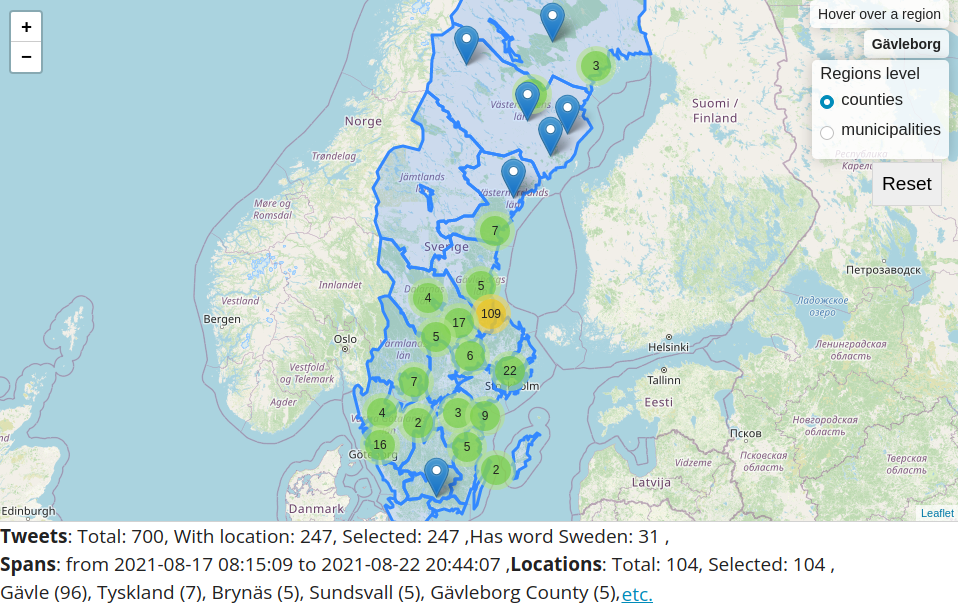
\includegraphics[width=14cm]{./images/gavle_map.png}
  \end{center}
  \caption{Map showing tweets about flood event in Gävleborg}
  \label{fig:gavle_map}
\end{figure}

\begin{figure}[H]
  \begin{center}
    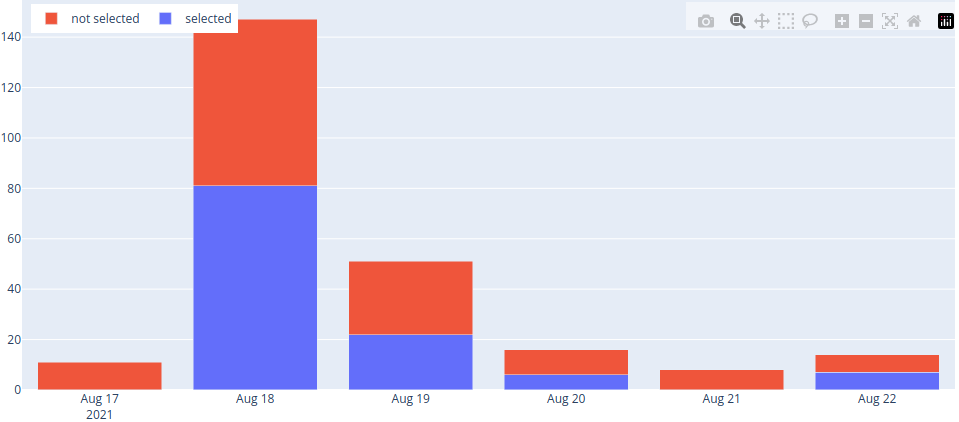
\includegraphics[width=12cm]{./images/gavle_histogram.png}
  \end{center}
  \caption{Histogram showing tweets about flood event in Gävleborg}
  \label{fig:gavle_histogram}
\end{figure}


After testing with several values for clustering properties, the ones shown in
Figure~\ref{fig:gavle_text_analysis_scatter_tables} identified a traffic disruption through the
bottom left cluster. The text in the tweets table (shown in
Figure~\ref{fig:gavle_text_analysias_tweets_table}) and the terms found by \ac{LDA} show that the
tweets discuss a traffic disruption caused by flooding, where \ac{LDA} is done with two topics only
because the number of selected tweets is too small.

\begin{figure}[H]
  \begin{center}
    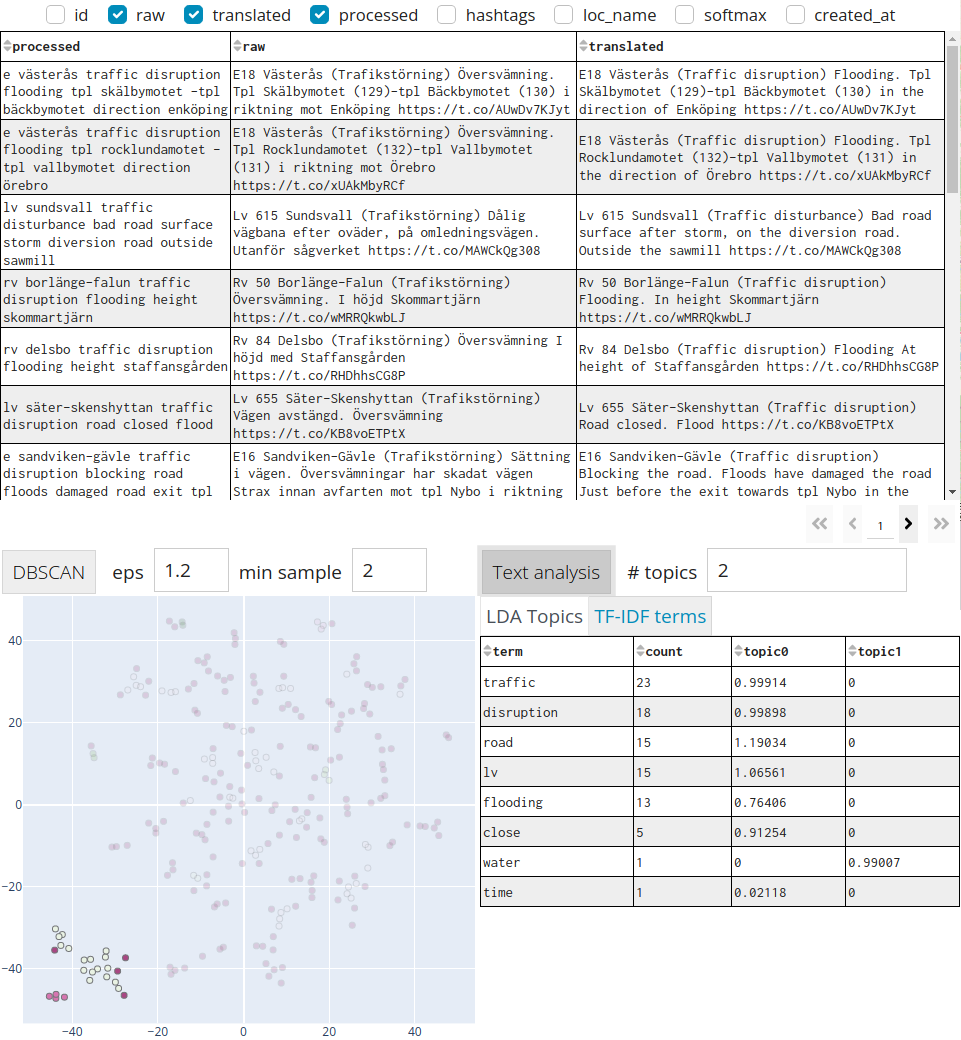
\includegraphics[width=\columnwidth, trim={0cm 0cm 0cm 14.5cm},clip]{./images/gavle_text_analysis.png}
  \end{center}
  \caption{Scatter plot, and \ac{LDA} table showing a cluster of tweets about flood event in Gävleborg}
  \label{fig:gavle_text_analysis_scatter_tables}
\end{figure}

\begin{figure}[H]
  \begin{center}
    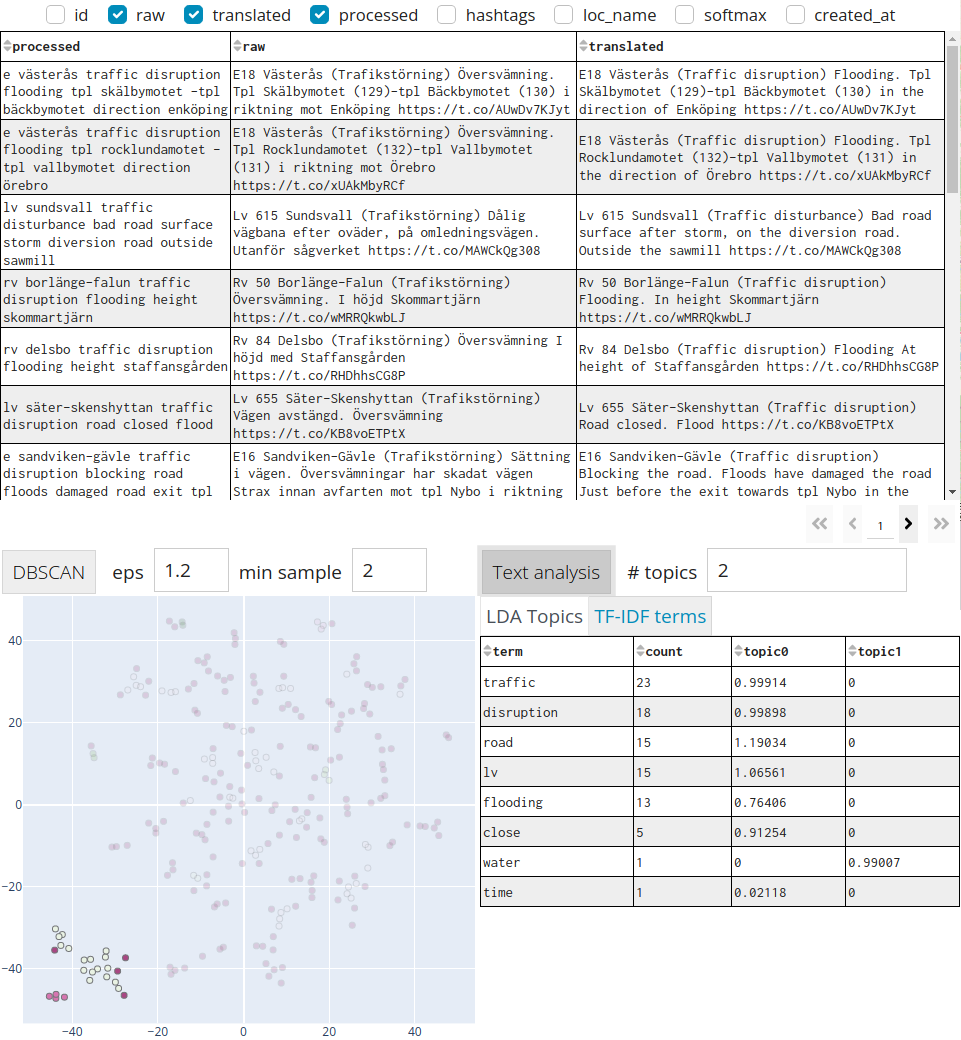
\includegraphics[width=\columnwidth, trim={0cm 13.1cm 0cm 0cm},clip]{./images/gavle_text_analysis.png}
  \end{center}
  \caption{Tweet table showing the selected cluster of tweets}
  \label{fig:gavle_text_analysias_tweets_table}
\end{figure}

Checking the map in Figure~\ref{fig:traffic_disruption_map} shows that the same tweets discuss
traffic disruptions in the southern parts of Gävleborg and Dalarna counties. Besides this, the text
analysis techniques didn't find anything interesting because the tweets are of small size and
composed of other elements besides text to capture their context.

\begin{figure}[H]
  \begin{center}
    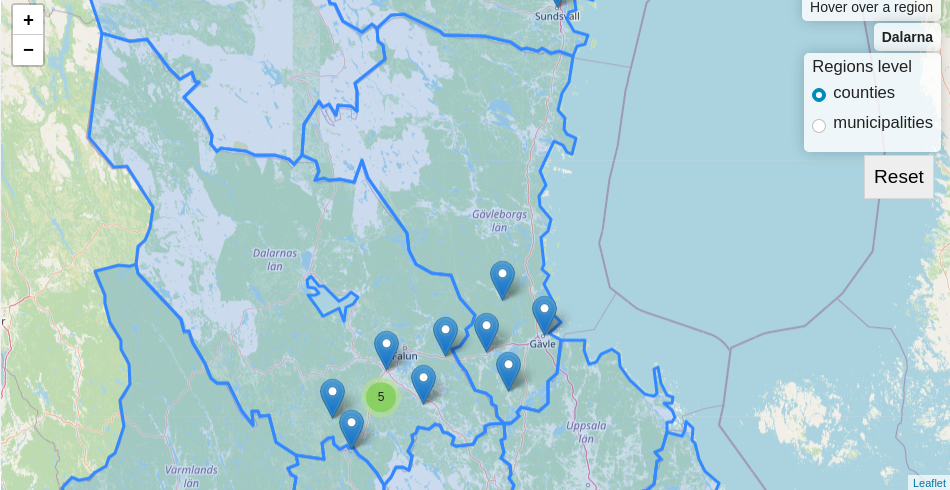
\includegraphics[width=14cm]{./images/traffic_disruption_map.png}
  \end{center}
  \caption{Map showing tweets discussing traffic disruption}
  \label{fig:traffic_disruption_map}
\end{figure}

\subsection{Gothenburg on 11 September 2019}

Heavy rain caused flooding in Gothenburg on 11 September
2019\footnote{https://floodlist.com/europe/sweden-flash-floods-gothenburg-september-2019}. After
extracting 315 tweets from Twitter's API and processing them, 243 were left, of which 117 were
classified as flood-relevant, of which 53 contained toponyms. The spatial and temporal distributions
of the plots in Figure~\ref{fig:gothenburg_map} show the true location and starting date of the
event, which is evident from the 18 flood-relevant tweets in Gothenburg county, of which 12 were
created on the 11th and three on the 12th. With that said, the location extraction step made an
error by identifying ``Spanien'', which was found in 16 tweets, as an isolated dwelling in
Stockholm; in fact, the tweets are discussing floods in the country
Spain\footnote{https://www.svt.se/nyheter/utrikes/stora-oversvamningar-har-drabbat-sodra-spanien}.
There are false negatives for classifying flood-relevant tweets, such as ``It was a little wet.
https://t.co/PcroA3s1A2'', where the tweet contains a \ac{URL} for an article mentioning the flood
event.

\begin{figure}[H]
  \begin{center}
    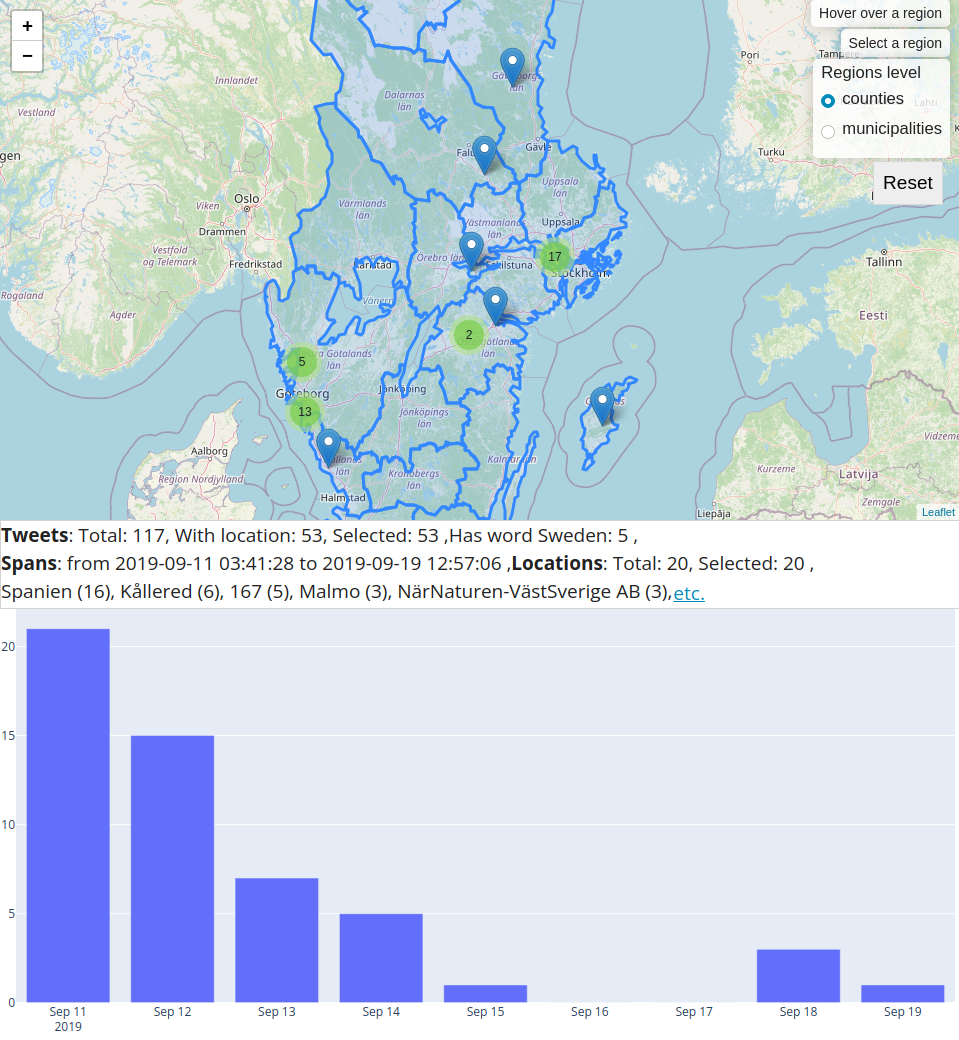
\includegraphics[width=12cm]{./images/gothenburg_floods.png}
  \end{center}
  \caption{Tweet table  showing tweets about flood event in Gothenburg}
  \label{fig:gothenburg_map}
\end{figure}

\subsection{Halland, Värmland and Västra Götaland on 18 and 19 August 2014}

On the 18 and 19 August 2014, Halland, Värmland and Västra Götaland counties had floods lasting four
days caused by heavy rain\footnote{https://floodlist.com/europe/four-days-floods-sweden}. After
extracting 1508 tweets from Twitter's API and processing them, 995 were left, of which 503 were
classified as flood-relevant, of which 226 contained locations in Sweden. The map in
Figure~\ref{fig:4days_floods} shows that Halland, Värmland, and Västra Götaland counties have 74,
41, and 27 tweets, respectively. The histogram shows 15 tweets created on the 18th, 67 on the 19th,
and 47 on the 20th.

\begin{figure}[H]
  \begin{center}
    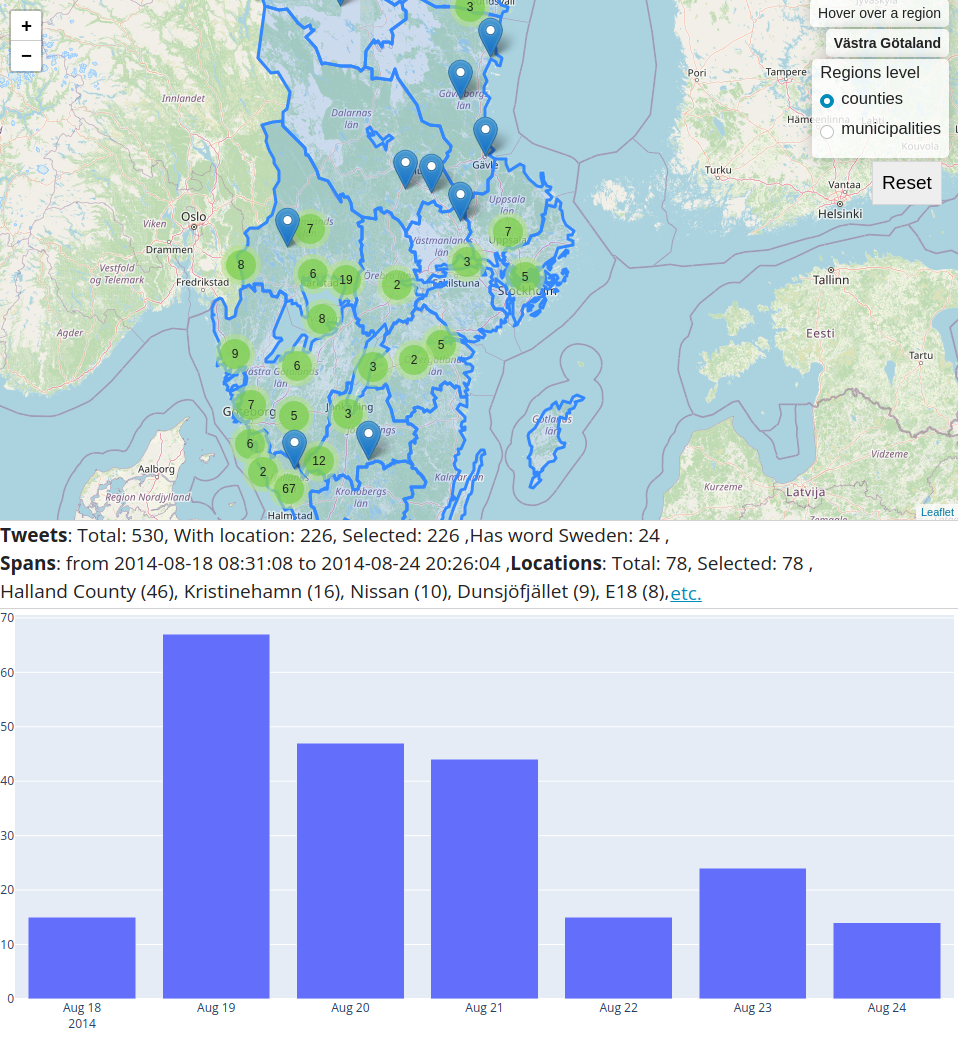
\includegraphics[width=13cm]{./images/4days_floods.png}
  \end{center}
  \caption{Map and histogram showing tweets about flood event in Swedish counties}
  \label{fig:4days_floods}
\end{figure}

The selected cluster in the scatter plot shown in Figure~\ref{fig:4days_text_analysis} contains tweets discussing \ac{SMHI}
warnings which is evident from the text in the tweets table and topic 1 in the \ac{LDA} table. 

\begin{figure}[H]
  \begin{center}
    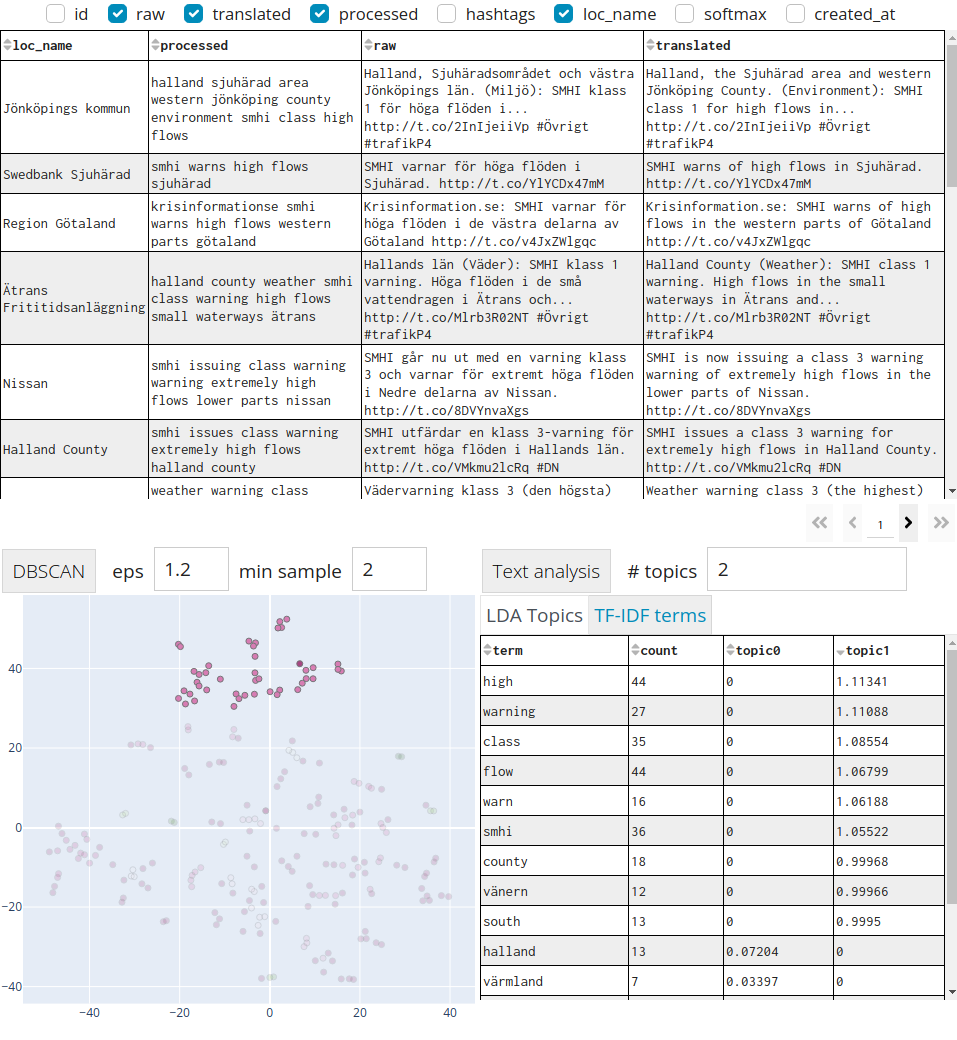
\includegraphics[width=\columnwidth]{./images/4days_text_analysis.png}
  \end{center}
  \caption{Tweet table, scatter plot, and \ac{LDA} table showing a selected cluster of tweets
  talking about \ac{SMHI} warnings}
  \label{fig:4days_text_analysis}
\end{figure}

Another cluster of tweets discusses traffic disruptions, as shown in Figure~\ref{fig:4days_text_analysis_traffic_disruption}, and the map in
Figure~\ref{fig:4days_text_analysis_traffic_disruption_map} shows the locations discussed in these tweets.

\begin{figure}[H]
  \begin{center}
    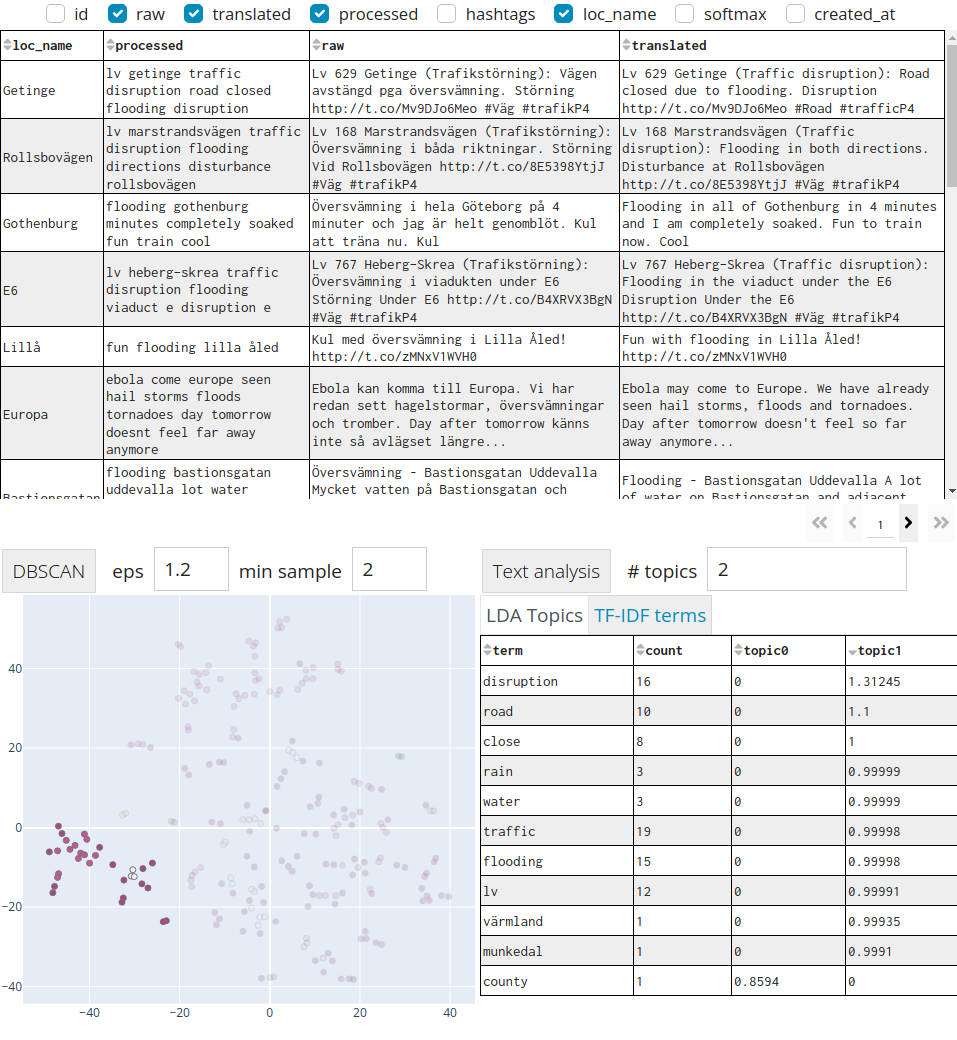
\includegraphics[width=\columnwidth]{./images/4days_text_analysis_traffic_disruption.png}
  \end{center}
  \caption{Tweet table, scatter plot, and \ac{LDA} table showing a selected cluster of tweets
  talking about traffic disruptions}
  \label{fig:4days_text_analysis_traffic_disruption}
\end{figure}

\begin{figure}[H]
  \begin{center}
    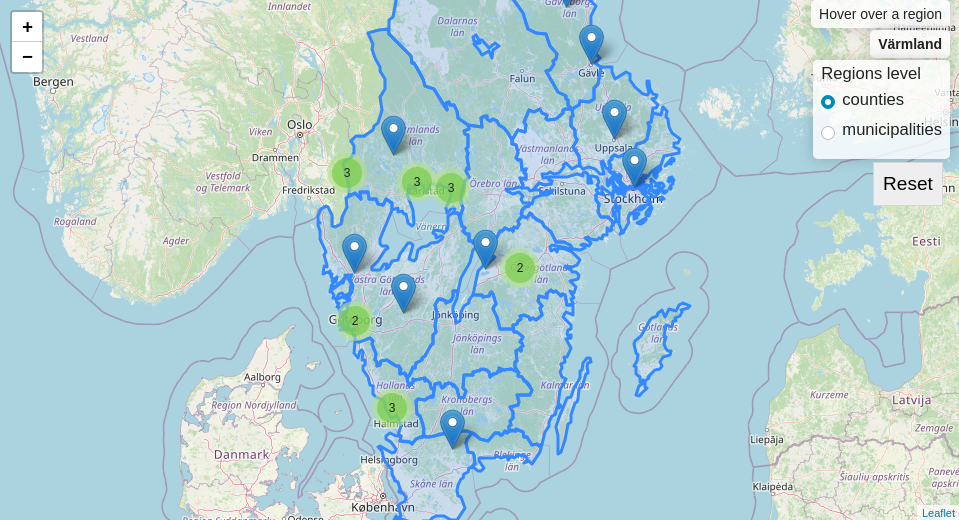
\includegraphics[width=\columnwidth]{./images/4days_text_analysis_traffic_disruption_map.png}
  \end{center}
  \caption{Map showing tweets mentioning traffic disruptions}
  \label{fig:4days_text_analysis_traffic_disruption_map}
\end{figure}
